\documentclass[slovak]{iamthesis}
% changle "slovak" to "english" for english version of the thesis

%----------------------------------------------------------------%
% THESIS DATA

% student name with title e.g. Ing. Martin Klaučo
\def\thesisauthor{Meno študenta} 

% year of submmiting to AIS
\def\thesisyear{rok}

% registration number generated by AIS e.g. 19990-50920
\def\thesisnumber{číslo práce} 

% thesis type: BACHELOR|MASTER|DISSERTATION or in slovak 
% BAKALÁRSKA|DIPLOMOVÁ|DIZERTAČNÁ
\def\thesistype{DIPLOMOVÁ}

% thesis title
\def\thesistitle{Názov práce}

% thesis supervisor including degrees e.g. Ing. Martin Klaučo, PhD.
\def\thesissupervisor{Ing. Martin Klaučo, PhD.}

% study field (translate to english if neccesarry) e.g. "Riadenie Procesov" or
% "Process Control"
\def\thesisprogram{Riadenie Procesov}

% Institute (translate to english if neccesary)
% e.g., "Institute of Information Engineering, Automation, and Mathematics"
\def\thesisinst{Oddelenie informatizácie a riadenia procesov}

% Title of the Acknowledgment
% For slovak write: "Poďakovanie" for English write: "Acknowledgment"
\def\thesisack{Poďakovanie}


% End THESIS DATA
%----------------------------------------------------------------%

%----------------------------------------------------------------%
%   Titles and other stuff                                       %
%----------------------------------------------------------------%
\author{\thesisauthor}
\title{\thesistitle}
\date{\today}
%\usepackage{layouts}
%\usepackage{layout}
%----------------------------------------------------------------%
%   Let the document begin                                       %
%----------------------------------------------------------------%
\begin{document}

% ---------------------------------------------------------------%
% The Frontmatter  !! Do NOT change the structure !!             % 
%----------------------------------------------------------------%

\coverpage

\frontmatter
\pagenumbering{roman}

% include assignment generated by AIS system
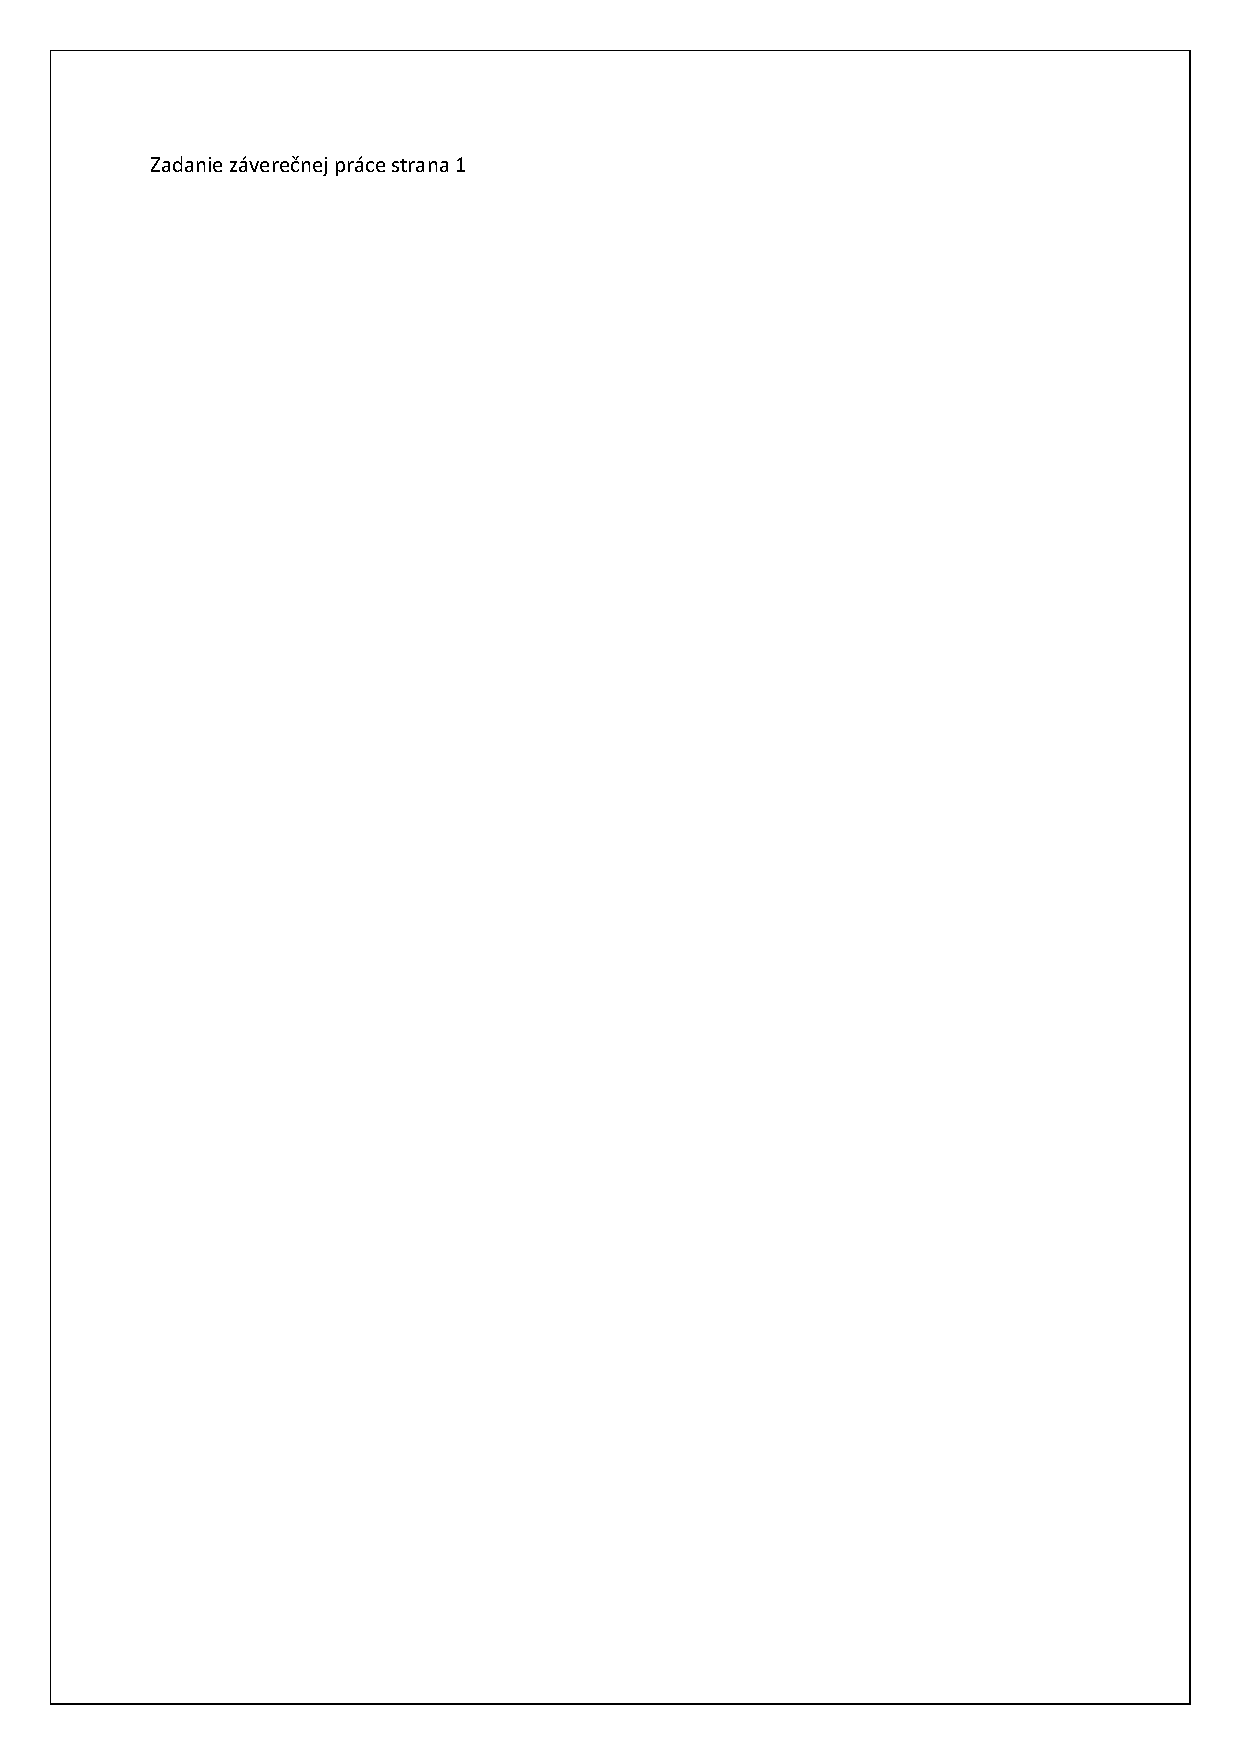
\includepdf[page=1]{content/assignment.pdf}
% use this command only if your assignment has more than 2 pages
% 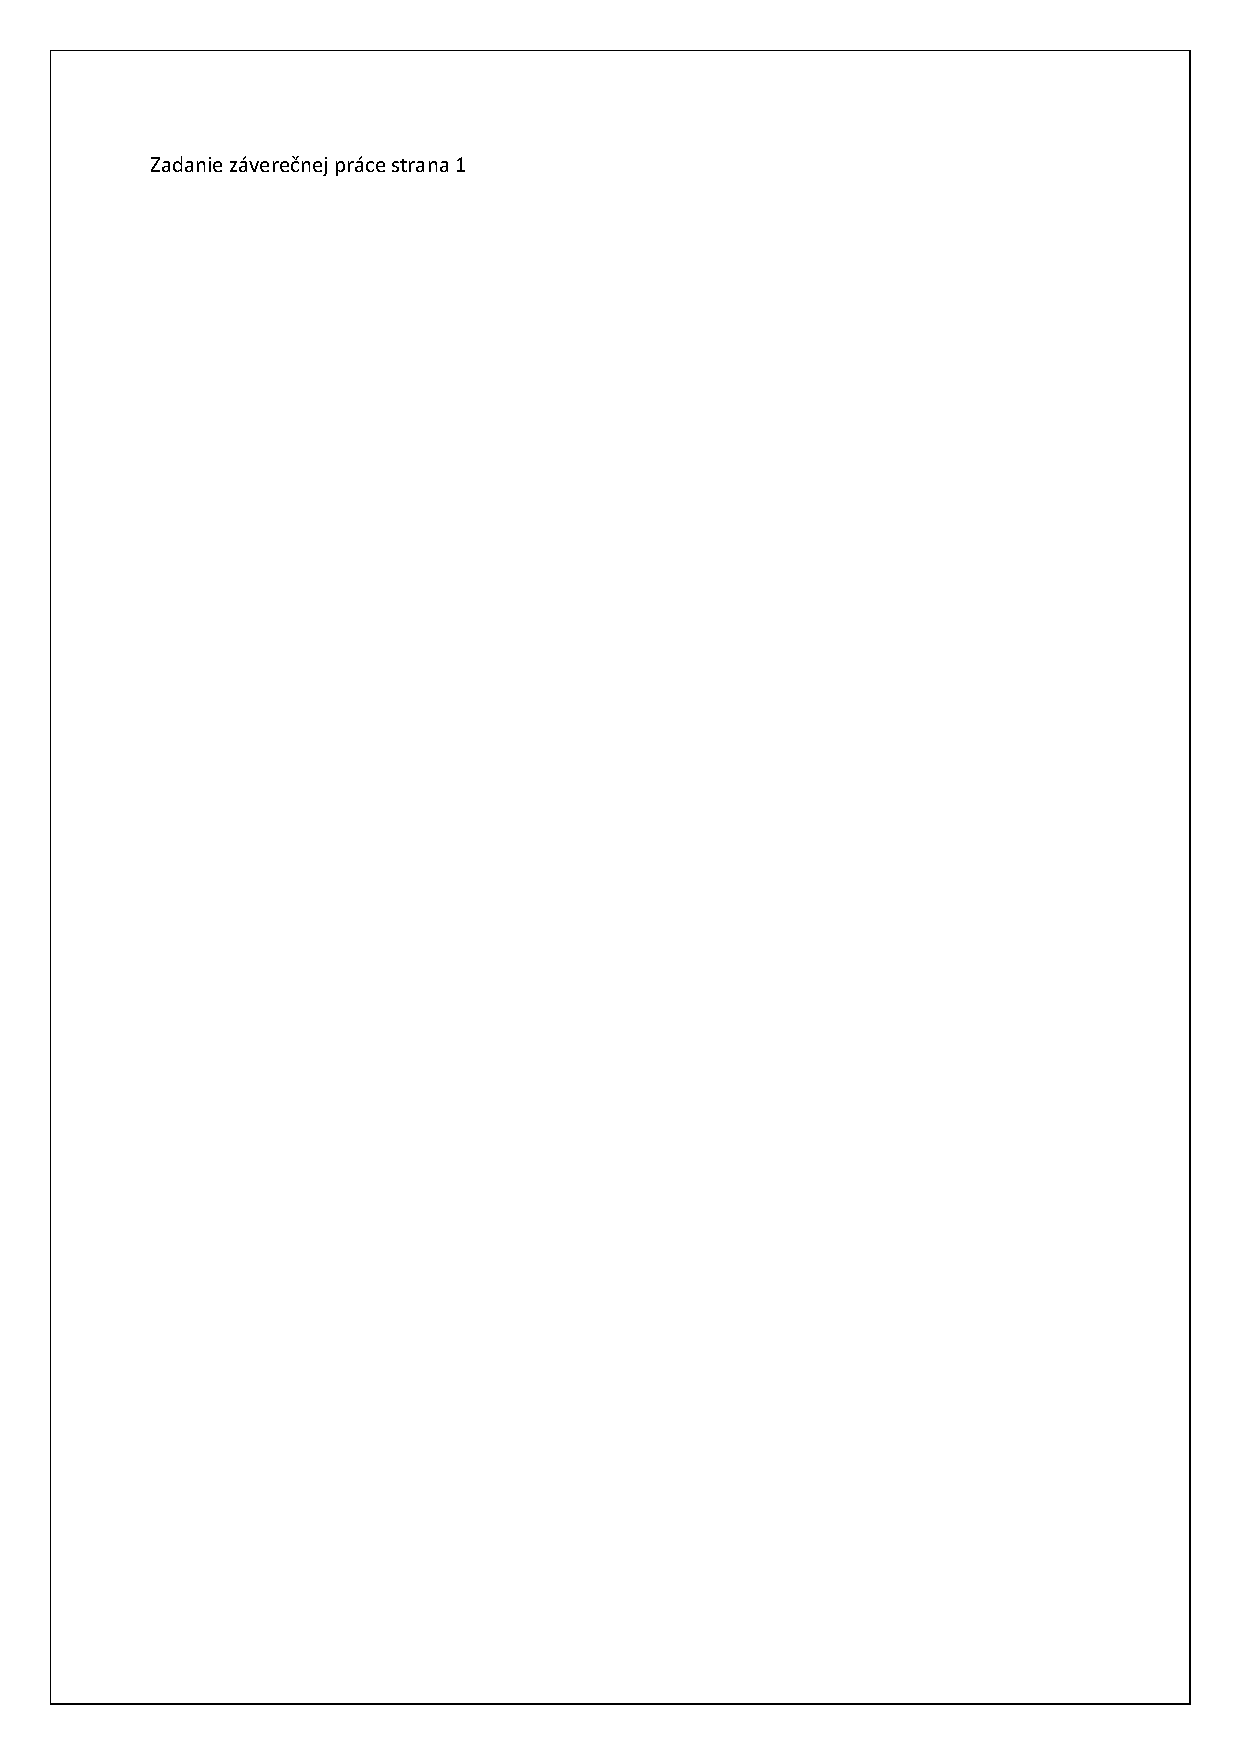
\includepdf[page=2]{content/assignment.pdf}


% do not remove following commands
% do not following commands
\chapter*{\thesisack}
\markboth{}{}
\addcontentsline{toc}{chapter}{\thesisack}
I would like to express my deep gratitude to my supervisor Ing. Martin Klaučo, PhD for his professional guidance, constructive recommendations and useful critiques of this thesis. My grateful thanks are also extended to my consultant Ing. Matúš Furka for his assistance and constructive suggestions during the development of this work. 


\chapter*{Abstract}
\markboth{}{}
\addcontentsline{toc}{chapter}{Abstract}
This work is dedicated to designing control strategies for the rotational inverted pendulum or Furuta’s pendulum. Those strategies are Linear-quadratic regulator (LQR) with the Swing-up controller, Model Predictive Control (MPC) method with the Swing-up controller and the Nonlinear Model Predictive Control (NMPC) strategy. Those controllers are designed in a computing environment MATLAB, for NMPC has used MATMPC toolbox as well as the CasADi toolbox. After verifying in simulations those controllers are used to control the real process.  


\chapter*{Abstrakt}
\markboth{}{}
\addcontentsline{toc}{chapter}{Abstrakt}
Slovenský abstrakt

\setcounter{tocdepth}{2}
\renewcommand{\baselinestretch}{0.1}\normalsize
\tableofcontents
\renewcommand{\baselinestretch}{1.1}\normalsize

% ----------------------------------------------------------------%
% The Mainmatter !! Do NOT change the structure!!                 %
% ----------------------------------------------------------------%
\mainmatter

% individual chapters should be included via a separate tex file, as shown in 
% here. When working in TexStudio (recomennded tool for Win and Mac) set the 
% main.tex as an Explicit root document, so you can compile even you are
% working on other chapter in other tex file.
%
% Open main.tex THEN click Options-> Root Document -> Set Current Document as
% Explicit Root

% introduction
\chapter{Introduction}
\label{ch:intro}

This \LaTeX template is intended for student writing their final theses at 
Faculty of Chemical and Food Technology. This chapter covers the basic setup of 
the LaTeX template as well as simple guidelines for high-quality typesetting. 
This template generates the thesis structure based on requirements. The 
template is intended for Slovak-writing as well as for English-writing students
\begin{verbatim}
\documentclass[english]{iamthesis}
% changle "english" to "slovak" for english version of the thesis
\end{verbatim}

The file structure of this LaTeX template
\begin{verbatim}
	|-- content/
	   |-- abstract_en.tex
	   |-- abstract_sk.tex
	   |-- introduction.tex	   
	   |-- assignment.pdf
	   |-- theory.tex
	   |-- conclusions.tex
	   |-- resume.tex
	|-- images/
		 |-- fchpt_logo_color.pdf
	|-- main.tex
	|-- bibfile.bib
\end{verbatim}

The root document is the \texttt{main.tex}. Here, the student must specify 
key-values of the thesis (lines 7 to 32), namely:
\begin{verbatim}
% student name with title e.g. Ing. Martin Klaučo
\def\thesisauthor{Students Name} 

% year of submmiting to AIS
\def\thesisyear{Year}

% registration number generated by AIS e.g. 19990-50920
\def\thesisnumber{Number} 

% thesis type: BACHELOR|MASTER|DISSERTATION or in slovak 
% BAKALÁRSKA|DIPLOMOVÁ|DIZERTAČNÁ
\def\thesistype{DIPLOMOVÁ}

% thesis title
\def\thesistitle{Title of the Thesis}

% thesis supervisor including degrees e.g. MSc. Ing. Martin Klaučo, PhD.
\def\thesissupervisor{Ing. Martin Klaučo, PhD.}

% study field (translate to english if neccesarry) e.g. 
% "Riadenie Procesov" or "Process Control"
\def\thesisprogram{Riadenie Procesov}

% Institute (translate to english if neccesary)
% e.g., "Institute of Information Engineering, Automation, and Mathematics"
\def\thesisinst{Ústav Automatizácie, Informatizácie a Riadenia Procesov}
\end{verbatim}

The file \texttt{assignment.pdf} is to be replaced by assignment generated by 
the AIS system.

The file \texttt{bibfile.bib} is to be expanded with your references. You can 
also provide your own bibfile. See command 
\texttt{\textbackslash{providebibliography}}.

\section{Typesetting Guidelines}
This template comes with predefined macros, help to ease up the typesetting of 
math. Refer to table~\ref{tab:commands} for examples.


Before submitting the thesis check if
\begin{itemize}
	\item all equations are referenced in the text (remember, you can refer only 
	to equation which was already written),
	\item all figures are referenced in the text (remember, figure must not 
	appear necessarily on the same page as you would like),
	\item all tables are referenced in the text (remember, figure must not 
		appear necessarily on the same page as you would like),
	\item every chapter, section or subsection must start with a paragraph,
	\item every chapter, section or subsection must end with text, not with 
	equation, nor with table or figure,
	\item if writing in English, check you grammar with free tool 
	\url{www.grammarly.com}.
\end{itemize}


\begin{table}[h]
	\centering
	\caption{Example of built-in commands}
	\label{tab:commands}
	\begin{tabular}{llp{5cm}}
		\toprule
			command & results & remark\\
		\midrule
		  \texttt{\textbackslash{ui\{F\}\{a\}}} &  $\ui{F}{a}$ & is used 
		  when the subindex ''a'' is part 
		  of notation\\
		  \texttt{\textbackslash{uis\{F\}\{a\}\{k\}}} &  $\uis{F}{a}{k}$ & is 
		  used  when  the  subindex ''a'' is  part  of notation and ''k'' is 
		  variable 
		  \\
		  \texttt{\textbackslash{Ts}} & $\Ts$ & sampling time \\[2pt]
		  \texttt{\textbackslash{lrp\{ \textbackslash{frac\{a\}\{b\}} \}}} & 
		  $\displaystyle\lrp{\frac{a}{b}}$& 
		  expandable parenthesis based on 
		  the expression size\\
		  \texttt{\textbackslash{lrb\{ \textbackslash{frac\{a\}\{b\}} \}}} & 
		  $\displaystyle\lrb{\frac{a}{b}}$& 
		  expandable brackets based on 
		  the expression size\\
		  \texttt{\textbackslash{dif\{f(x)\}\{x\}}} & 
		  $\displaystyle\dif{f(x)}{x}$& \\[10pt]
		  \texttt{\textbackslash{diff\{f(x, y)\}\{x\}}} & 
		  $\displaystyle\diff{f(x,y )}{x}$& \\[10pt]
		  \texttt{\textbackslash{diffxy\{f(x,y)\}\{x\}\{y\}}} & 
		  $\displaystyle\diffxy{f(x, y)}{x}{y}$& \\[10pt]
		  \texttt{\textbackslash{diffat\{f(x,y)\}\{x\}\{x=0\}}} & 
		  $\displaystyle\diffat{f(x, y)}{x}{x=0}$& \\[10pt]
		  \texttt{\textbackslash{difat\{f(x,y)\}\{x\}\{x=0\}}} & 
		  $\displaystyle\difat{f(x, y)}{x}{x=0}$& \\[10pt]
		  \texttt{\textbackslash{dt\{f(t)\} } } & $\displaystyle\dt{f(t)}$  & \\
		\bottomrule
	\end{tabular}
	% the "\displaystyle" command for increased font size of the math expression 
	%  in table
\end{table}

Example of citing literature~\cite{boyd:book:2009:cvx}.

% theory
\chapter{Theory}

\section{Furuta's Pendulum}

Rotational inverted pendulum or Furuta’s pendulum composes of two main parts: motor-driven arm, which rotates in the horizontal plane and a pendulum, attached to that arm, which freely rotates in the vertical plane. The system is underactuated and extremely nonlinear due to the gravitational forces and the coupling arising from the Coriolis and centripetal forces. The schematic representation of the pendulum is shown in \ref{furuta}
\begin{figure}[h]
	\centering
	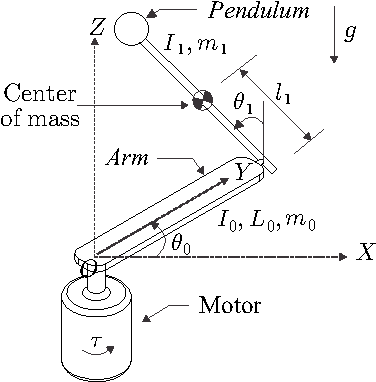
\includegraphics[width=.6\linewidth]{images/furuta}
	\caption{Furuta's Pendulum}
	\label{furuta}
\end{figure}
\newpage
The symbols in the figure indicate the following:
\begin{itemize}
	\item \textbf{$g$} - gravitational acceleration [\si{\metre\per\square\second}]
	\item \textbf{$m_0$} - mass of arm [\si{\kilogram}]
	\item \textbf{$m_1$} - mass of pendulum [\si{\kilogram}]
	\item \textbf{$L_0$} - length of arm [\si{\metre}]
	\item \textbf{$L_1$} - length of pendulum [\si{\metre}]
	\item \textbf{$l_1$} - location of the pendulums center of mass [\si{\metre}]
	\item \textbf{$I_0$} - moment of inertia of arm [\si{\kilogram\per\square\metre}]
	\item \textbf{$I_1$} - moment of inertia of pendulum [\si{\kilogram\per\square\metre}]
	\item \textbf{$\theta_0$} - arm angle [\si{\radian}]
	\item \textbf{$\theta_1$} - pendulum angle [\si{\radian}]
	\item \textbf{$\tau$} - motor torque [\si{\volt}]
\end{itemize}
\subsection{State-Space Representation}
To obtain the state representation of the process we must define our state variables first:
\begin{equation}
	\begin{bmatrix}
	x_1 & x_2 & x_3 & x_4
	\end{bmatrix}^\intercal = 
	\begin{bmatrix}
	\theta_0 & \dot{\theta_0} & \theta_1 & \dot{\theta_1}
	\end{bmatrix}^\intercal
\end{equation}
Control variable:
\begin{equation} u = \tau \end{equation}
Then we can write our state equations:
\begin{subequations}
\begin{equation}\dot{x_1} = \dot{\theta_0} \end{equation}
\begin{equation}\dot{x_2} = \frac{\gamma(\epsilon\dot{\theta_0}^2+\rho)-\delta(\tau+\beta\dot{\theta_1}^2-\sigma\dot{\theta_0}\dot{\theta_1})}{\gamma^2-\alpha\delta}\end{equation}
\begin{equation}\dot{x_3} = \dot{\theta_1}\end{equation}
\begin{equation}\dot{x_4} = \frac{\gamma(\tau+\beta\dot{\theta_1}^2-\sigma\dot{\theta_0}\dot{\theta_1})-\alpha(\epsilon\dot{\theta_0}^2+\rho)}{\gamma^2-\alpha\delta}\end{equation}
\end{subequations}
where
\begin{equation}\alpha = I_0+L_0^2m_1+l_1^2m_1\sin^2\theta_1\end{equation}
\begin{equation}\beta = L_0m_1l_1\sin\theta_1 \end{equation}
\begin{equation}\gamma = L_0m_1l_1\cos\theta_1\end{equation}
\begin{equation}\delta = I_1+l_1^2m_1\end{equation}
\begin{equation}\epsilon = l^2_1m_1\sin\theta_1\cos\theta_1\end{equation}
\begin{equation}\rho = m_1gl_1\sin\theta_1\end{equation}
\begin{equation}\tau = 2l^2_1m_1\sin\theta_1\cos\theta_1\end{equation}
Now these non-linear differential equations we can write in the form of matrices:
\begin{equation}\label{nonlinmodel}
\begin{bmatrix}
\dot{x_1} \\ \dot{x_2} \\ \dot{x_3} \\ \dot{x_4}
\end{bmatrix} = \begin{bmatrix}
\dot{\theta_0}\\
\frac{\gamma(\epsilon\dot{\theta_0}^2+\rho)-\delta(\tau+\beta\dot{\theta_1}^2-\sigma\dot{\theta_0}\dot{\theta_1})}{\gamma^2-\alpha\delta}\\
\dot{\theta_1}\\
 \frac{\gamma(\tau+\beta\dot{\theta_1}^2-\sigma\dot{\theta_0}\dot{\theta_1})-\alpha(\epsilon\dot{\theta_0}^2+\rho)}{\gamma^2-\alpha\delta}
\end{bmatrix}
\end{equation}
or:
\begin{equation}\dot{x} = f(x,u) =\begin{bmatrix}f_1(x,u)\\f_2(x,u)\\f_3(x,u)\\f_4(x,u)\end{bmatrix} \end{equation}
So that’s our non-linear dynamic model of the process. But only the NMPC controller is able to operate with such a model.  So, to make that model suitable for LQR and MPC controller we can approximate that non-linear model by a linear model as follows:
\begin{equation}\dot{x} = Ax + Bu\end{equation}
And the constant matrices are derived as:
\begin{equation}
A = \begin{bmatrix}
\frac{\partial f_1(x,u)}{\partial x_1}&\frac{\partial f_1(x,u)}{\partial x_2}&\frac{\partial f_1(x,u)}{\partial x_3}&\frac{\partial f_1(x,u)}{\partial x_4}\\
\frac{\partial f_2(x,u)}{\partial x_1}&\frac{\partial f_2(x,u)}{\partial x_2}&\frac{\partial f_2(x,u)}{\partial x_3}&\frac{\partial f_2(x,u)}{\partial x_4}\\
\frac{\partial f_3(x,u)}{\partial x_1}&\frac{\partial f_3(x,u)}{\partial x_2}&\frac{\partial f_3(x,u)}{\partial x_3}&\frac{\partial f_3(x,u)}{\partial x_4}\\
\frac{\partial f_4(x,u)}{\partial x_1}&\frac{\partial f_4(x,u)}{\partial x_2}&\frac{\partial f_4(x,u)}{\partial x_3}&\frac{\partial f_4(x,u)}{\partial x_4}
\end{bmatrix}
\end{equation}
respektive:
\begin{equation}
	A =\begin{bmatrix}0&1&0&0\\
	0&0&\frac{-gL_0l_1^2m_1^2}{(m_1L_0^2+I_0)(m_1l_1^2+I_1)-L_0^2l_1^2m_1^2}&0\\
	0&0&0&1\\
	0&0&\frac{gl_1m_1(m_1L_0^2+I_0)}{(m_1L_0^2+I_0)(m_1l_1^2+I_1)-L_0^2l_1^2m_1^2}&0
	\end{bmatrix}
\end{equation}
\begin{equation}B = \begin{bmatrix}
\frac{\partial f_1(x,u)}{\partial u}\\\frac{\partial f_2(x,u)}{\partial u}\\\frac{\partial f_3(x,u)}{\partial u}\\\frac{\partial f_4(x,u)}{\partial u}
\end{bmatrix}=\begin{bmatrix}
0\\ 
\frac{m_1L_1^2+I_1}{(m_1L_0^2+I_0)(m_1l_1^2+I_1)-L_0^2l_1^2m_1^2}\\0\\
\frac{-L_0l_1m_1}{(m_1L_0^2+I_0)(m_1l_1^2+I_1)-L_0^2l_1^2m_1^2}
\end{bmatrix}\end{equation}
\begin{equation}C = \begin{bmatrix}0&0&1&0\end{bmatrix}\end{equation}
\begin{equation}D = 0\end{equation}
The linearized equations of motion for the simplified system are now could be derived for two equilibrium positions: upright and downward. The reason is that at the downward position the system's output, which is the position of the pendulum, has a stable point at “$+\pi$” and “$-\pi$”, while at the upright position system has no stable point.\\

The model, obtained by linearization around the upright operation point, is used for fulfilling the main control objective, which is stabilizing the pendulum at the upright position. The second model is used to simulate process behavior during initial excitation by a Swing-up controller.
\section{Controller Synthesis}
\subsection{LQR design}
The Linear Quadratic Regulator (LQR) is a well-known method that provides optimally controlled feedback gains to enable the closed-loop stable and high performance design of systems.
\begin{equation}
\begin{split}
\dot{x} &= Ax + Bu\\
y &= Cx, C=I^{n \times n}
\end{split}
\end{equation}
which requires  full-state feedback (all n states are measurable).
The feedback gain is a matrix K and the feedback control law takes the form:
\begin{equation}
	u = -Kx
\end{equation}
Than closed-loop system dynamics can be written:
\begin{equation}
\dot{x} = (A-BK)x
\end{equation}
So there appears condition that poles of $(A-BK)$ must be in in stable, suitably-damped locations in the complex plane.
\subsubsection{Derivation of LQR}
Towards a generic procedure for solving optimal control problems, we derive a methodology based on the calculus of variations. The problem statement for a fixed final time $t_f$ is:
\begin{equation}
\begin{split}
	J = \min_{u}& \quad \Phi(t_f)+\frac{1}{2}\int\limits_{t_0}^{t_f}L(x(t),u(t),t)\;dt\\
	s.t.&\quad  \dot{x} = f(x(t),u(t),t)\\
	& \quad x(t_0) = x_0
	\end{split}
\end{equation}
In the case of the Linear Quadratic Regulator (with zero terminal cost), we set  $\Phi(x(t_f))=0$, and $L = x^\intercal Qx+u^\intercal Ru$ solve the new optimization problem
\begin{equation}
J=\min_{u}  \frac{1}{2}\int\limits_{t_0}^{t_f}x^\intercal Qx+u^\intercal Ru\;dt
\end{equation}
Where $Q$ and $R$ are positive semidefinite weighting matrices for states and control input respectively.
Now we define new variable $H$ as:
\begin{equation}
H = \frac{1}{2}(x\intercal Qx + u^\intercal Ru)+\lambda^\intercal(Ax + Bu)
\end{equation}

As we are looking for minimum, we apply the condition, that $\frac{\partial H(x,u,\lambda)}{\partial u}$ is equal to zero.
\begin{equation}
	\frac{\partial H(x,u,\lambda)}{\partial u} = Ru + B^\intercal\lambda = 0
\end{equation}
then:
\begin{equation}
u = -R^{-1}B^\intercal\lambda
\end{equation}
where
\begin{equation}
\lambda = Px
\end{equation}
and finally
\begin{equation}
u = -R^{-1}B^\intercal Px
\end{equation}
And that is our optimal control law for full-state feedback LQR. Matrix $P$ is calculated by solving Riccati equation in continuous time:
\begin{equation}
Q + A^\intercal P + PA - PBR^{-1}B^\intercal P = 0
\end{equation}
\subsection{MPC controller design}
MPC uses a model of the system to make predictions about the system’s future behavior. MPC solves an online optimization algorithm to find the optimal control action that drives the predicted output to the reference. MPC can handle MIMO systems that may have interactions between their inputs and outputs. It can also handle input and output constraints. MPC has preview capability; it can incorporate future reference information into the control problem to improve controller performance.
\subsubsection{MPC formulation}
MPC controller requires the model of the system in the discrete time formulation that
is used to predict systems behavior in the future:
\begin{equation}
	\begin{split}
	&x_{k+1} = Ax_k + Bu_k\\
	&y_k = Cx_k
	\end{split}
\end{equation}
State predictions: 
\begin{equation}
\begin{split}
\hat{x}_{k+1} &= Ax_k + Bu_k\\
\hat{x}_{k+2} &= A\hat{x}_{k+1} + Bu_{k+1}\\
&= A^2x_k + ABu_k + Bu_{k+1}\\
\hat{x}_{k+3} &= A\hat{x}_{k+2} + Bu_{k+2}\\
&= A^3x_k + A^2Bu_k + ABu_{k+1} + Bu_{k+2}\\
&\vdots\\
\hat{x}_{k+N} &= A^Nx_k+\sum_{j=k}^{k+N-1}A^jBu_{k+N-j-1}
\end{split}
\end{equation}
Output Predictions:
\begin{equation}
\begin{split}
\hat{y}_{k+1} &= C\hat{x}_{k+1}\\
			  &= CAx_k + CBu_k\\
\hat{y}_{k+2} &= C\hat{x}_{k+2}\\
			  &= CA^2x_k + CABu_k + CBu_{k+1}\\
			  \hat{y}_{k+2} &= C\hat{x}_{k+2}\\
			  &= CA^3x_k + CA^2Bu_k + CABu_{k+1} + CBu_{k+2}
\end{split}
\end{equation}
Now we can obtain predictive system model:
\begin{equation}
	\begin{bmatrix}
	\hat{y}_{k+1}\\\hat{y}_{k+2}\\ \vdots\\ \hat{y}_{k+N}
	\end{bmatrix} = \begin{bmatrix}CA\\CA^2\\ \vdots \\ CA^N\end{bmatrix}x_k + \begin{bmatrix}CB& 0&\cdots&0\\
	CAB&CB&\cdots&0\\
	\vdots&\vdots&\ddots&\vdots\\
	CA^{N-1}&CA^{N-2}&\cdots&CB\end{bmatrix}\begin{bmatrix}u_k\\u_{k+1}\\\vdots\\u_{k+N-1}\end{bmatrix}
\end{equation}
respektive:
\begin{equation}
	\hat{Y} = Y_0 + GU
\end{equation}
And now the whole optimization problem could be written as a QP problem with constrains:
\begin{equation}\label{mpcformulation}
\begin{split}
J = \min_{u}& \sum_{k}^{k+N}x^\intercal Q_xx+u^\intercal Q_uu\\
s.t.&\quad  x_{k+1} = Ax_k + Bu_k\\
&\quad  y_{k} = Cx_k\\
& \quad u_{min}\leq u_k\leq u_{max}
\end{split}
\end{equation}
Where $Q_x$ and $Q_u$ are positive semidefinite weighting matrices for states and control input respectively.
By solving that optimization problem we get the optimal value for control input for every simulation step.
\subsection{Swing-Up controller design}
For initial excitation of the system we use the energy-based swing-up controller. The strategy with this controller is that we increase the amplitude of swings by increasing the energy of the system with every swing. The energy is added by controlling arms movements and depends on the actual energy of the pendulum. The actual energy of the pendulum can be calculated from the actual position of the pendulum and its velocity: 
\begin{equation}
E = \frac{m_1gl_1}{2}((\frac{\dot{\theta_1}}{\omega_0})^2+\cos\theta_1 - 1)
\end{equation}
Than the control law has following form:
\begin{equation}
	u = k_vEsign(\dot{\theta_1}\cos\theta_1)
\end{equation}
Where element $sign(\dot{\theta_1}\cos\theta_1)$ determines direction i which the force will be applied and $k_vE$ is the gain of the controller.









% conclusions
\chapter{Conclusions}
In this thesis, we have developed a control strategies to control a complex nonlinear oscillator what the Furuta pendulum is. The main task was to perform a Swing-Up control of the pendulum, with its stabilization at the upright position in an optimal way. But before we could proceed to the control strategies and control attempts, the mathematical dynamic model of the pendulum must be obtained first. For that purpose, a Lagrangian formulation of the system dynamics of the mechanical system was used. The Lagrangian formulation requires the construction of Lagrangian and Euler-Lagrange equations. As the Furuta pendulum has two degrees of freedom, two Euler-Lagrange equations were constructed. Then, by solving those equations, two equations of motion for both the Arm And the Pendulum were obtained. Further from those equations of motion, the nonlinear continuous-time State-Space dynamic model of the pendulum was derived. Then by linearizing that nonlinear model at the upright operation point, the linear dynamic model was acquired.

The next part of the thesis is a theoretical foundation for the individual controllers, used to control the pendulum. There are in total three controllers a Model Predictive Controller, an Energy-Shaping controller, and a Nonlinear Model Predictive Controller. For MPC was shown how to transform a problem of state regulation to the origin, to the standard Quadratic Programming problem. For Energy-Shaping controller was discussed the control law, which allows implementing such a state-feedback controller. For NMPC was shown how to solve a Nonlinear Programming problem by a numerical method, called Sequential Quadratic Programming.

The main task of the thesis is to perform Heuristic Swing-Up control and Optimal Swing-Up control of the pendulum. For Heuristic Swing-Up control an MPC and Energy-Shaping controllers were used. Initially, a Swing-Up controller is used to bring the pendulum in a range around the upright operating point, where the linear dynamic model is valid. Then the active controller switches to MPC, which further stabilizes the pendulum at the upright position. For the Optimal Swing-Up control the NMPC strategy was used. NMPC was designed through the \textsc{Matmpc} toolbox.

All controllers were designed and tested in \textsc{Matlab}. The obtained results are closer discussed in individual sections of the respective chapter.

% Appendices (Prílohy) comment by "%" if not neccesary
\appendix
\chapter{Resumé}
\label{ch:resume}

Resumé v slovenčine, sa píše v prípade, že záverečná práca ja napísaná v 
anglickom jazyku. Rozsah resumé tvorí 5-10\% rozsahu diplomovej práce.

%----------------------------------------------------------------%
%  The Backmatter !! Do NOT change the structure!!               %
%----------------------------------------------------------------%
% Bibliography to TOC
% do not remove
\backmatter
\providebibliography
\bibliography{bibfile}

%----------------------------------------------------------------%
%   The end of the document                                      %
%----------------------------------------------------------------%
\end{document}
